\section{Factorial designs: Round 2}

Designs with more than one independent variable refer to designs where
the experimenter manipulates at least two independent variables.
Consider the light-switch example from the previous chapter. Imagine you
are trying to figure out which of two light switches turns on a light.
The dependent variable is the light (we measure whether it is on or
off). The first independent variable is light switch \#1, and it has two
levels, up or down. The second independent variable is light switch \#2,
and it also has two levels, up or down. When there are two independent
variables, each with two levels, there are four total conditions that
can be tested. We can describe these four conditions in a 2x2 table.

\begin{longtable}[]{@{}ccc@{}}
\toprule
& Switch 1 Up & Switch 1 Down\tabularnewline
\midrule
\endhead
Switch 2 Up & Light ? & Light ?\tabularnewline
Switch 2 Down & Light ? & Light ?\tabularnewline
\bottomrule
\end{longtable}

This kind of design has a special property that makes it a factorial
design. That is, the levels of each independent variable are each
manipulated across the levels of the other indpendent variable. In other
words, we manipulate whether switch \#1 is up or down when switch \#2 is
up, and when switch numebr \#2 is down. Another term for this property
of factorial designs is ``fully-crossed''.

It is possible to conduct experiments with more than independent
variable that are not fully-crossed, or factorial designs. This would
mean that each of the levels of one independent variable are not
necessarilly manipulated for each of the levels of the other independent
variables. These kinds of designs are sometimes called unbalanced
designs, and they are not as common as fully-factorial designs. An
example, of an unbalanced design would be the following design with only
3 conditions:

\begin{longtable}[]{@{}ccc@{}}
\toprule
& Switch 1 Up & Switch 1 Down\tabularnewline
\midrule
\endhead
Switch 2 Up & Light ? & Light ?\tabularnewline
Switch 2 Down & Light ? & NOT MEASURED\tabularnewline
\bottomrule
\end{longtable}

Factorial designs are often described using notation such as AXB, where
A= the number of levels for the first independent variable, and B = the
number of levels for the second independent variable. The fully-crossed
version of the 2-light switch experiment would be called a 2x2 factorial
design. This notation is convenient because by multiplying the numbers
in the equation we can find the number of conditions in the design. For
example 2x2 = 4 conditions.

More complicated factorial designs have more indepdent variables and
more levels. We use the same notation describe these designs. The number
for each variable represents the number of levels for that variable, and
the number of numbers in the equation represents the number of
variables. So, a 2x2x2 design has three independent variables, and each
one has 2 levels, for a total of 2x2x2=6 conditions. A 3x3 design has
two independent variables, each with three levels, for a total of 9
conditions. Designs can get very complicated, such as a 5x3x6x2x7
experiment, with five independent variables, each with differing numbers
of levels, for a total of 1260 conditions. If you are considering a
complicated design like that one, you should consider how to simplify
it.

\subsection{2x2 Factorial designs}\label{x2-factorial-designs}

For simplicity, we will focus mainly on 2x2 factorial designs. As with
simple designs with only one independent variable, factorial designs
have the same basic empirical question. Did the manipulation cause a
change in the measurement? However, 2x2 designs have more than one
manipulation, so there is more than one way that a change in measurement
can be observed. So, we end up asking the basic empirical question more
than once.

More specifically, the analysis of factorial designs are split into two
parts: main effects and interactions. Main effects are occur when the
levels of one independent variable cause a change in the dependent
variable. In a 2x2 design, there are two independent variables, so there
are two possible main effects: the main effect of independent variable
1, and the main effect of independent variable 2. An interaction occurs
when the effect of one independent variable \emph{depends} on the levels
of the other independent variable. My experience in teaching the concept
of main effects and interactions is that they are confusing. So, I
expect that these definitions will not be very helpful, and although
they are clear and precise, they only become helpful as definitions
after you understand the concepts\ldots{}so they are not useful for
explaining the concepts. To explain the concepts we will go through
several different kinds of examples.

To briefly add to the confusion, or perhaps to illustrate why these two
concepts can be confusing, we will look at the eight possible outcomes
that could occur in a 2x2 factorial experiment.

\begin{longtable}[]{@{}cccc@{}}
\toprule
Possible outcome & IV1 main effect & IV2 main effect &
Interaction\tabularnewline
\midrule
\endhead
1 & yes & yes & yes\tabularnewline
2 & yes & no & yes\tabularnewline
3 & no & yes & yes\tabularnewline
4 & no & no & yes\tabularnewline
5 & yes & yes & no\tabularnewline
6 & yes & no & no\tabularnewline
7 & no & yes & no\tabularnewline
8 & no & no & no\tabularnewline
\bottomrule
\end{longtable}

In the table, a yes means that there was statistically significant
difference for one of the main effects or interaction, and a no means
that there was not a statisically significant difference. As you can
see, just by adding one more independent variable, the number of
possible outcomes quickly become more complicated. When you conduct a
2x2 design, the task for analysis is to determine which of the 8
possibilites occured, and then explain the patterns for each of the
effects that occurred. That's a lot of explaining to do.

\subsection{Main effects}\label{main-effects}

Main effects occur when the levels of an independent variable cause
change in the measurement or dependent variable. There is one possible
main effect for each independent variable in the design. When we find
that independent variable did cause change, then we say there was a main
effect. When we find that the independent variable did not cause change,
then we say there was no main effect.

The simplest way to understand a main effect is to pretend that the
other independent variables do not exist. If you do this, then you
simply have a single-factor design, and you are asking whether that
single factor caused change in the measurement. For a 2x2 experiment,
you do this twice, once for each independent variable.

Let's consider a silly example to illustrate an important property of
main effects. In this experiment the dependent variable will be height
in inches. The independent variables will be shoes and hats. The shoes
independent variable will have two levels: wearing shoes vs.~no shoes.
The hats independent variable will have two levels: wearing a hat
vs.~not wearing a hat. The experiment will provide the shoes and hats.
The shoes add 1 inch to a person's height, and the hats add 6 inches to
a person's height. Further imagine that we conduct a within-subjects
design, so we measure each person's height in each of the fours
conditions. Before we look at some example data, the findings from this
experiment should be pretty obvious. People will be 1 inch taller when
they wear shoes, and 6 inches taller when they where a hat. We see this
in the example data from 10 subjects presented below:

\begin{longtable}[]{@{}rrrr@{}}
\toprule
NoShoes\_NoHat & Shoes\_NoHat & NoShoes\_Hat & Shoes\_Hat\tabularnewline
\midrule
\endhead
56 & 57 & 62 & 63\tabularnewline
57 & 58 & 63 & 64\tabularnewline
58 & 59 & 64 & 65\tabularnewline
57 & 58 & 63 & 64\tabularnewline
57 & 58 & 63 & 64\tabularnewline
57 & 58 & 63 & 64\tabularnewline
58 & 59 & 64 & 65\tabularnewline
57 & 58 & 63 & 64\tabularnewline
57 & 58 & 63 & 64\tabularnewline
57 & 58 & 63 & 64\tabularnewline
\bottomrule
\end{longtable}

The mean heights in each condition are:

\begin{longtable}[]{@{}lr@{}}
\toprule
NoShoes\_NoHat & 57.1\tabularnewline
Shoes\_NoHat & 58.1\tabularnewline
NoShoes\_Hat & 63.1\tabularnewline
Shoes\_Hat & 64.1\tabularnewline
\bottomrule
\end{longtable}

To find the main effect of the shoes manipulation we want to find the
mean height in the no shoes condition, and compare it to the mean height
of the shoes condition. To do this, we \emph{collapse}, or average over
the observations in the hat conditions. For example, looking only at the
no shoes vs.~shoes conditions we see the following averages for each
subject.

\begin{longtable}[]{@{}rr@{}}
\toprule
NoShoes & Shoes\tabularnewline
\midrule
\endhead
59 & 60\tabularnewline
60 & 61\tabularnewline
61 & 62\tabularnewline
60 & 61\tabularnewline
60 & 61\tabularnewline
60 & 61\tabularnewline
61 & 62\tabularnewline
60 & 61\tabularnewline
60 & 61\tabularnewline
60 & 61\tabularnewline
\bottomrule
\end{longtable}

The group means are:

\begin{longtable}[]{@{}lr@{}}
\toprule
NoShoes & 60.1\tabularnewline
Shoes & 61.1\tabularnewline
\bottomrule
\end{longtable}

As expected, we see that the average height is 1 inch taller when
subjects wear shoes vs.~do not wear shoes. So, the main effect of
wearing shoes is to add 1 inch to a person's height.

We can do the very same thing to find the main effect of hats. Except in
this case, we find the average heights in the no hat vs.~hat conditions
by averaging over the shoe variable.

\begin{longtable}[]{@{}rr@{}}
\toprule
NoHat & Hat\tabularnewline
\midrule
\endhead
56.5 & 62.5\tabularnewline
57.5 & 63.5\tabularnewline
58.5 & 64.5\tabularnewline
57.5 & 63.5\tabularnewline
57.5 & 63.5\tabularnewline
57.5 & 63.5\tabularnewline
58.5 & 64.5\tabularnewline
57.5 & 63.5\tabularnewline
57.5 & 63.5\tabularnewline
57.5 & 63.5\tabularnewline
\bottomrule
\end{longtable}

The group means are:

\begin{longtable}[]{@{}lr@{}}
\toprule
NoHat & 57.6\tabularnewline
Hat & 63.6\tabularnewline
\bottomrule
\end{longtable}

As expected, we the average height is 6 inches taller when the subjects
wear a hat vs.~do not wear a hat. So, the main effect of wearing hats is
to add 1 inch to a person's height.

Instead of using tables to show the data, let's use some bar graphs.
First, we will plot the average heights in all four conditions.

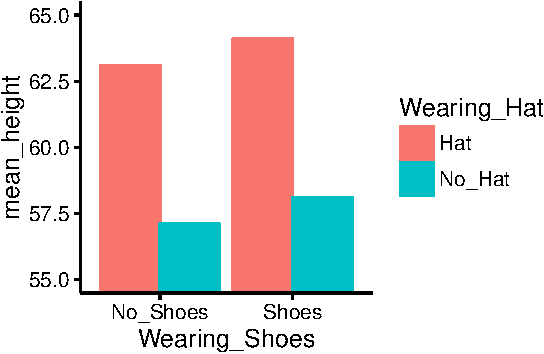
\includegraphics{Factorial_files/figure-latex/unnamed-chunk-7-1}

Some questions to ask yourself are 1) can you identify the main effect
of wearing shoes in the figure, and 2) can you identify the main effet
of wearing hats in the figure. Both of these main effects can be seen in
the figure, but they aren't fully clear. You have to do some visual
averaging.

Perhaps the most clear is the main effect of wearing a hat. The red bars
show the conditions where people wear hats, and the green bars show the
conditions where people do not wear hats. For both levels of the wearing
shoes variable, the red bars are higher than the green bars. That is
easy enough to see. More specifically, in both cases, wearing a hat adds
exactly 6 inches to the height, no more no less.

Less clear is the main effect of wearing shoes. This is less clear
because the effect is smaller so it is harder to see. How to find it?
You can look at the red bars first and see that the red bar for
no\_shoes is slightly smaller than the red bar for shoes. The same is
true for the green bars. The green bar for no\_shoes is slightly smaller
than the green bar for shoes.

\begin{figure}
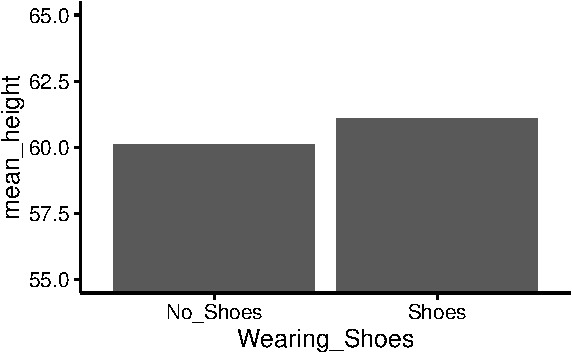
\includegraphics[width=.5\linewidth]{Factorial_files/figure-latex/unnamed-chunk-8-1} \end{figure}

\begin{figure}
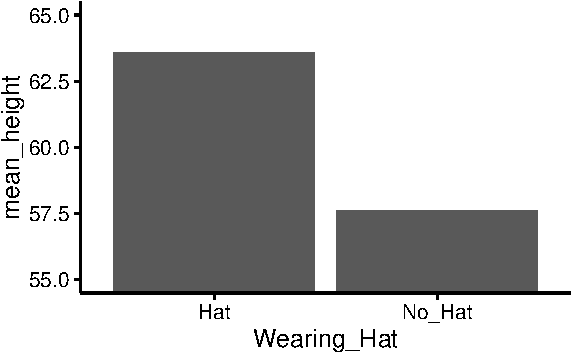
\includegraphics[width=.5\linewidth]{Factorial_files/figure-latex/unnamed-chunk-8-2} \end{figure}

Data from 2x2 designs is often present in graphs like the one above. An
advantage of these graphs is that they display means in all four
conditions of the design. However, they do not clearly show the two main
effects. Someone looking at this graph alone would have to guesstimate
the main effects. Or, in addition to the main effects, a researcher
could present two more graphs, one for each main effect (however, in
practice this is not commonly done because it takes up space in a
journal article, and with practice it becomes second nature to ``see''
the presence or absence of main effects in graphs showing all of the
conditions). If we made a separate graph for the main effect of shoes we
should see a difference of 1 inch between conditions. Similarly, if we
made a separate graph for the main effect of hats then we should see a
difference of 6 between conditions. Examples of both of those graphs
appear in the margin.

Why have we been talking about shoes and hats? These independent
variables are good examples of variables that are truly independent from
one another. Neither one influences the other. For example, shoes with a
1 inch sole will always add 1 inch to a person's height. This will be
true no matter whether they wear a hat or not, and no matter how tall
the hat is. In other words, the effect of wearing a shoe does not depend
on wearing a hat. More formally, this means that the shoe and hat
independent variables do not interact. It would be very strange if they
did interact. It would mean that the effect of wearing a shoe on height
would depend on wearing a hat. This does not happen in our universe. But
in some other imaginary universe, it could mean, for example, that
wearing a shoe adds 1 to your height when you do not wear a hat, but
adds more than 1 inch (or less than 1 inch) when you do wear a hat. This
thought experiment will be our entry point into discussing interactions.
A take-home message before we begin is that some independent variables
(like shoes and hats) do not interact; however, there are many other
independent variables that do.

\subsection{Interactions}\label{interactions}

Interactions occur when the effect of an independent variable depends on
the levels of the other independent variable. As we discussed above,
some independent variables are independent from one another and will not
produce interactions. However, other combinations of independent
variables are not independent from one another and they produce
interactions. Remember, independent variables are always manipulated
independently from the measured variable (see margin note), but they are
not necessarilly independent from each other.

\begin{marginfigure}
These ideas can be confusing if you think that the word ``independent''
refers to the relationship between independent variables. However, the
term ``independent variable'' refers to the relationship between the
manipulated variable and the measured variable. Remember, ``independent
variables'' are manipulated independently from the measured variable.
Specifically, the levels of any independent variable do not change
because we take measurements. Instead, the experimenter changes the
levels of the independent variable and then observes possible changes in
the measures.
\end{marginfigure}

There are many simple examples of two independent variables being
dependent on one another to produce an outcome. Consider driving a car.
The dependent variable (outcome that is measured) could be how far the
car can drive in 1 minute. Independent variable 1 could be gas (has gas
vs.~no gas). Independent variable 2 could be keys (has keys vs.~no
keys). This is a 2x2 design, with four conditions.

\begin{longtable}[]{@{}ccc@{}}
\toprule
& Gas & No Gas\tabularnewline
\midrule
\endhead
Keys & can drive & x\tabularnewline
No Keys & x & x\tabularnewline
\bottomrule
\end{longtable}

Importantly, the effect of the gas variable on driving depends on the
levels of having a key. Or, to state it in reverse, the effect of the
key variable on driving depends on the levesl of the gas variable.
Finally, in plain english. You need the keys and gas to drive.
Otherwise, there is no driving.

\subsection{What makes a people
hangry?}\label{what-makes-a-people-hangry}

To continue with more examples, let's consider an imaginary experiment
examining what makes people hangry. You may have been hangry before.
It's when you become highly irritated and angry because you are very
hungry\ldots{}hangry. I will propose an experiment to measure conditions
that are required to produce hangriness. The pretend experiment will
measure hangriness (we ask people how hangry they are on a scale from
1-10, with 10 being most hangry, and 0 being not hangry at all). The
first independent variable will be time since last meal (1 hour vs.~5
hours), and the second independent variable will be how tired someone is
(not tired vs very tired). I imagine the data could look something the
following bar graph.

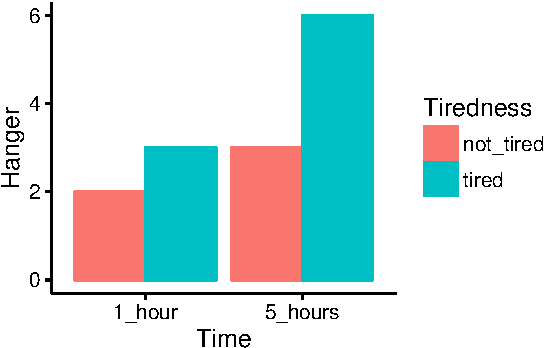
\includegraphics{Factorial_files/figure-latex/unnamed-chunk-10-1}

The graph shows clear evidence of two main effects,
\emph{and an interaction}. There is a main effect of time since last
meal. Both the bars in the 1 hour conditions have smaller hanger ratings
than both of the bars in the 5 hour conditions. There is a main effect
of being tired. Both of the bars in the ``not tired'' conditions are
smaller than than both of the bars in the ``tired'' conditions. What
about the interaction?

Remember, an interaction occurs when the effect of one independent
variable depends on the level of the other independent variable. We can
look at this two ways, and either way shows the presence of the very
same interaction. First, does the effect of being tired depend on the
levels of the time since last meal? Yes. Look first at the effect of
being tired only for the ``1 hour condition''. We see the red bar
(tired) is 1 unit lower than the green bar (not\_tired). So, there is an
effect of 1 unit of being tired in the 1 hour condition. Next, look at
the effect of being tired only for the ``5 hour'' condition. We see the
red bar (tired) is 3 units lower than the green bar (not\_tired). So,
there is an effect of 3 units for being tired in the 5 hour condition.
Clearly, the size of the effect for being tired depends on the levels of
the time since last meal variable. We call this an interaction.

The second way of looking at the interaction is to start by looking at
the other variable. For example, does the effect of time since last meal
depend on the levels of the tired variable? The answer again is yes.
Look first at the effect of time since last meal only for the red bars
in the ``not tired'' condition. The red bar in the 1 hour condition is 1
unit smaller than the red bar in the 5 hour condition. Next, look at the
effect of time since last meal only for the green bars in the ``tired''
condition. The green bar in the 1 hour condition is 3 units smaller than
the green bar in the 5 hour condition. Again, the size of the effect of
time since last meal depends on the levels of the tired variable.No
matter which way you look at the interaction, we get the same numbers
for the size of the interaction effect, which is 2 units (a difference
between 3 and 1 = 2). The interaction suggests that something special
happens when people are tired and haven't eaten in 5 hours. In this
condition, they can become very hangry. Whereas, in the other
conditions, there are only small increases in being hangry.

\subsection{Identifying main effects and
interactions}\label{identifying-main-effects-and-interactions}

Research findings are often presented to readers using graphs or tables.
For example, the very same pattern of data can be displayed in a bar
graph, line graph, or table of means. These different formats can make
the data look different, even though the pattern in the data is the
same. An important skill to develop is the ability to identify the
patterns in the data, regardless of the format they are presented in.
Some examples of bar and line graphs are presented in the margin, and
two example tables are presented below. Each format displays the same
pattern of data.

\begin{marginfigure}
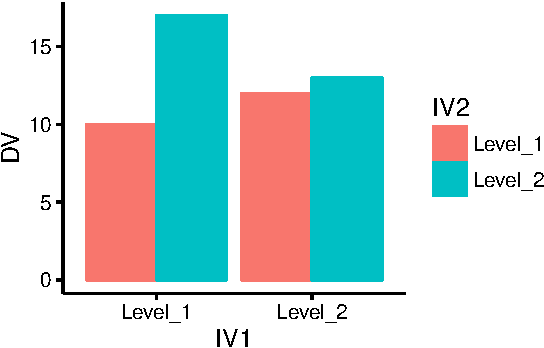
\includegraphics{Factorial_files/figure-latex/unnamed-chunk-11-1} \end{marginfigure}
\begin{marginfigure}
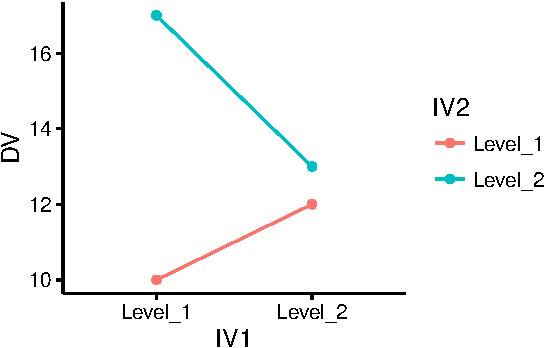
\includegraphics{Factorial_files/figure-latex/unnamed-chunk-11-2} \end{marginfigure}

\begin{longtable}[]{@{}lll@{}}
\toprule
DV I & V1 I & V2\tabularnewline
\midrule
\endhead
10 & Level\_1 & Level\_1\tabularnewline
12 & Level\_2 & Level\_1\tabularnewline
17 & Level\_1 & Level\_2\tabularnewline
13 & Level\_2 & Level\_2\tabularnewline
\bottomrule
\end{longtable}

\begin{verbatim}
##          df$IV2
## df$IV1    Level_1 Level_2
##   Level_1      10      17
##   Level_2      12      13
\end{verbatim}

After you become comfortable with interpreting data in these different
formats, you should be able to quickly identify the pattern of main
effects and interactions. For example, you would be able to notice that
all of these graphs and tables show evidence for two main effects and
one interaction.

As an exercise toward this goal, we will first take a closer look at
extracting main effects and interactions from tables. This exercise will
how the condition means are used to calculate the main effects and
interactions. Consider the table of condition means below.

\begin{longtable}[]{@{}cccc@{}}
\toprule
& & IV1 &\tabularnewline
\midrule
\endhead
& & A & B\tabularnewline
IV2 & 1 & 4 & 5\tabularnewline
& 2 & 3 & 8\tabularnewline
\bottomrule
\end{longtable}

\subsection{Main effects}\label{main-effects-1}

Main effects are the differences between the means of single independent
variable. Notice, this table only shows the condition means for each
level of all independent variables. So, the means for each IV must be
calculated. The main effect for IV1 is the comparison between level A
and level B, which involves calculating the two column means. The mean
for IV1 Level A is (4+3)/2 = 3.5. The mean for IV1 Level B is (5+8)/2 =
6.5. So the main effect is 3 (6.5 - 3.5). The main effect for IV2 is the
comparison between level 1 and level 2, which involves calculating the
two row means. The mean for IV2 Level 1 is (4+5)/2 = 4.5. The mean for
IV2 Level 2 is (3+8)/2 = 5.5. So the main effect is 1 (5.5 - 4.5). The
process of computing the average for each level of a single independent
variable, always involves collapsing, or averaging over, all of the
other conditions from other variables that also occured in that
condition

\subsection{Interactions}\label{interactions-1}

Interactions ask whether the effect of one independent variable depends
on the levels of the other independent variables. This question is
answered by computing difference scores between the condition means. For
example, we look the effect of IV1 (A vs.~B) for both levels of of IV2.
Focus first on the condition means in the first row for IV2 level 1. We
see that A=4 and B=5, so the effect IV1 here was 5-4 = 1. Next, look at
the condition in the second row for IV2 level 2. We see that A=3 and
B=8, so the effect of IV1 here was 8-3 = 5. We have just calculated two
differences (5-4=1, and 8-3=5). These difference scores show that the
size of the IV1 effect was different across the levels of IV2. To
calculate the interaction effect we simply find the difference between
the difference scores, 5-1=4. \emph{In general, if the difference
between the difference scores is different, then there is an interaction
effect.}

\subsection{Example bar graphs}\label{example-bar-graphs}

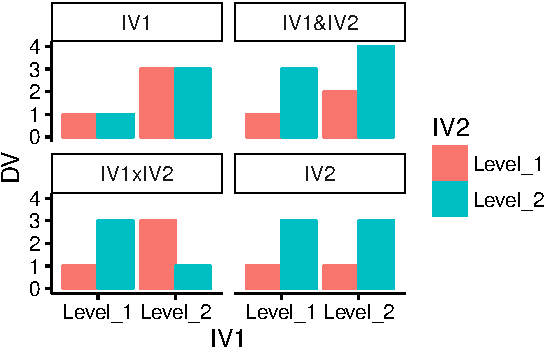
\includegraphics{Factorial_files/figure-latex/unnamed-chunk-13-1}

The IV1 graph shows a main effect only for IV1 (both red and green bars
are lower for level 1 than level 2). The IV1\&IV2 graphs shows main
effects for both variables. The two bars on the left are both lower than
the two on the right, and the red bars are both lower than the green
bars. The IV1xIV2 graph shows an example of a classic cross-over
interaction. Here, there are no main effects, just an interaction. There
is a difference of 2 between the green and red bar for Level 1 of IV1,
and a difference of -2 for Level 2 of IV1. That makes the differences
between the differences = 4. Why are their no main effects? Well the
average of the red bars would equal the average of the green bars, so
there is no main effect for IV2. And, the average of the red and green
bars for level 1 of IV1 would equal the average of the red and green
bars for level 2 of IV1, so there is no main effect. The bar graph for
IV2 shows only a main effect for IV2, as the red bars are both lower
than the green bars.

\subsection{Example line graphs}\label{example-line-graphs}

You may find that the patterns of main effects and interaction looks
different depending on the visual format of the graph. The exact same
patterns of data plotted up in bar graph format, are plotted as line
graphs for your viewing pleasure. Note that for the IV1 graph, the red
line does not appear because it is hidden behind the green line (the
points for both numbers are identical).

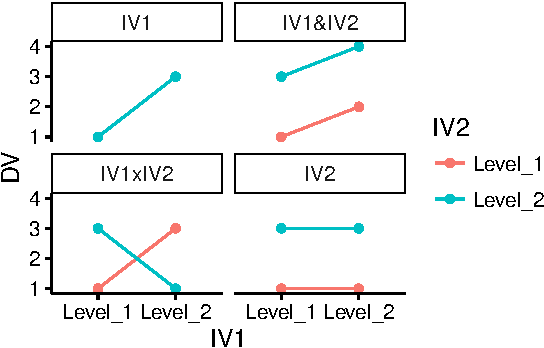
\includegraphics{Factorial_files/figure-latex/unnamed-chunk-14-1}

\subsection{Interpreting main effects and
interactions}\label{interpreting-main-effects-and-interactions}

The presence of an interaction can sometimes change how we interpet main
effects. For example, a really strong interaction can produce the
appearance of a main effect, even though when we look at the data most
people would agree the main effect is not there.

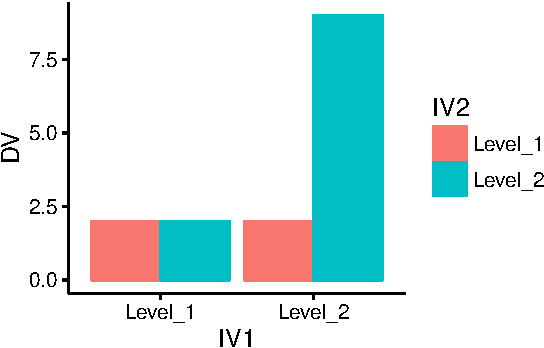
\includegraphics{Factorial_files/figure-latex/unnamed-chunk-15-1}

In the above graph there is clearly an interaction. IV2 has no effect
under level 1 of IV1 (e.g., the red and green bars are the same). IV2
has a large effect under level 2 of IV2 (the red bar is 2 and the green
bar is 9). So, the interaction effect is a total of 7. Are there any
main effects? This is a debatable question. Consider the main effect for
IV1. The mean for level 1 is (2+2)/2 = 2, and the mean for level 2 is
(2+9)/2 = 5.5. There is a difference between the means of 3.5, which is
consistent with a main effect. Consider, the main effect for IV2. The
mean for level 1 is again (2+2)/2 = 2, and the mean for level 2 is again
(2+9)/2 = 5.5. Again, there is a difference between the means of 3.5,
which is consistent with a main effect. What is going on here is that
the process of averagin over conditions that we use to compute main
effects is causing a main effect to appear, even though we don't really
see clear evidence of main effects.

Clear evidence of a main effect typically refers to cases where there is
a consistent additive influence. For example, if there really was a main
effect of IV1, then both red and green bars for level 2 should be
higher, not just one of them. In other words, the effect of IV1 did not
uniformly raise or lower the means across all of the other conditions.
For this reason, the main effects that we observed by performing the
calculation are really just an interaction in disguise.

The next example shows a case where it would be more appropriate to
conclude that the main effects and the interaction were both real.

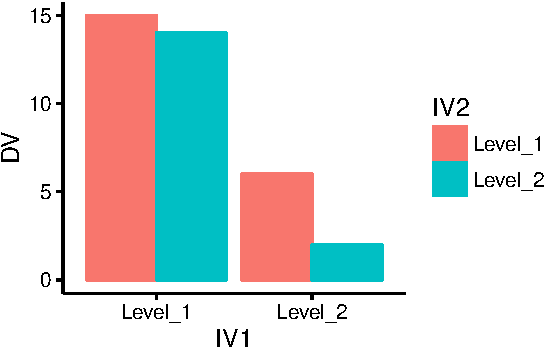
\includegraphics{Factorial_files/figure-latex/unnamed-chunk-16-1}

Can you spot the interaction right away? The difference between red and
green bars is small for level 1 of IV1, but large for level 2. The
differences between the differences are different, so there is an
interaction. But, we also see clear evidence of two main effects. For
example, both the red and green bars for IV1 level 1 are higher than IV1
Level 2. And, both of the red bars (IV2 level 1) are higher than the
green bars (IV2 level 2).


